\documentclass{beamer}
\usepackage[utf8]{inputenc}
\usepackage[T1]{fontenc}
\usepackage[sfdefault]{FiraSans}
\usepackage{verbatim}
\usepackage{graphicx}
\usetheme{Antibes}
\usecolortheme{dolphin}

\title{Communicating AI Effectively}
\author{Lynn Bradshaw}
\date{10 August 2019}

\begin{document}
  \begin{frame}
    \maketitle
  \end{frame}

  \begin{frame}
    \frametitle{Outline}
    \tableofcontents[pausesections]
  \end{frame}

  \section{Shameless Advertisement of the Presentation Medium}

  \subsection{The Advertisement}

  \begin{frame}
    \frametitle{How This Presentation Was Made}
    \begin{itemize}
      \item I can't say I'm not partial towards my tools.
      \pause
      \item This presentation was created in the typesetting system \LaTeX,
        using the Beamer presentation class.
      \pause
      \item Because \LaTeX{} is text, I was able to take advantage of Vim's
        advantages.
      \pause
      \item In \LaTeX, content is king.
      \item There are however word processor-like frontends and other editors.
      \pause
      \item I'm a slob but I appreciate attention to detail in typography.
    \end{itemize}
  \end{frame}

  \subsection{Here's What It Looks Like}

  \begin{frame}
    \frametitle{The Header}
    \begin{center}
      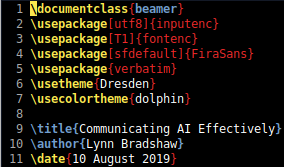
\includegraphics[width=0.9\textwidth]{latex-header.png}
    \end{center}
  \end{frame}

  \begin{frame}
    \frametitle{Part of an Earlier Draft}
    \begin{center}
      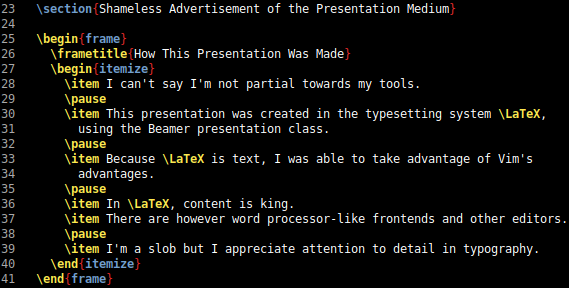
\includegraphics[width=0.9\textwidth]{latex-section-and-frame.png}
    \end{center}
  \end{frame}

  \section{Don't Just Take My Word for It}

  \begin{frame}
    \frametitle{Don't Just Take My Word for It}

    \begin{itemize}
      \item This presentation will necessarily be opinionated.
      \pause
      \item Unfortunately I am fallible.
      \pause
      \item I may be right a lot of the time but you can't win them all.
      \pause
      \item (\ldots{}but pray that what I have to say about Skynet being
        unrealistic is true.)
      \pause
      \item Further research is heavily recommended.
      \pause
      \item At the end of the presentation, feel free to challenge or add to
        anything I've said here.
    \end{itemize}
  \end{frame}

  \section{Taxonomy of AI and Its Uses}

  \subsection{Why This Approach?}

  \begin{frame}
    \frametitle{Why This Approach?}

    \begin{itemize}
      \item Basically people more or less know what ``artificial
        intelligence'' is. The problem is that they don't know the details.
      \pause
      \item Compare biological taxonomy: knowing what animals, loosely
        speaking, are but not knowing the difference between the classes
        \textit{Annelida} (segmented worms) and \textit{Aves} (birds).
      \pause
      \item My taxonomy traces the historical development of the field, offering
        further understanding.
      \pause
      \item Having said this, there are different ways the field can be split
        up and none is decisively the best one.
      \pause
      \item (N.b.: to avoid making issues more complicated than they already
        are I will leave out robotics almost entirely.)
    \end{itemize}
  \end{frame}

  \subsection{Traditional Methods}

  % Check the Russell and Norvig text and historical material
  \begin{frame}
    \frametitle{Foundation of the Field}
    \begin{itemize}
      \item Occurred during the Dartmouth Summer Project of 1954.
      \pause
      \item Groundbreaking but preceded by decades and even centuries by
        precedents of notions about thinking or otherwise capable automata.
      \pause
      \item Core founders considered to be John McCarthy, Marvin Minsky,
        Herbert Simon and Allen Newell.
    \end{itemize}
  \end{frame}

  \begin{frame}
    \frametitle{The Results}
    \begin{itemize}
      \item The fraught name!
      \pause
      \item Departure from early experiments in neural networks (yes!) towards
        symbol processing.
      \pause
      \item The stunning early success of Logic Theorist.
      \pause
      \item The ball was now rolling.
    \end{itemize}
  \end{frame}

  \begin{frame}
    \frametitle{Other Developments in the 50s and 60s}
    \begin{itemize}
      \item Early (finicky) character recognition.
      \pause
      \item Perceptrons.
      \pause
      \item Early statistical methods, including nearest neighbor.
      \pause
      \item Heuristic problem-solving methods, including General Problem
        Solver and some fairly decent checkers and chess programs.
      \pause
      \item (Very crappy) machine translation.
      \pause
      \item Semantic networks.
    \end{itemize}
  \end{frame}

  \begin{frame}
    \frametitle{Some Very Ominous Quotes About AI from This Era}

    \begin{itemize}
      \item ``[If] one could devise a successful chess machine, one would seem
        to have penetrated to the core of human intellectual endeavor.'' ---
        Allen Newell, Cliff Shaw and Herbert Simon, 1958
      \item ``Machines will be capable, within twenty years, of doing any work
        a man can do.'' --- Herbert Simon, 1965
      \item ``Within a generation \ldots the problem of creating `artificial
        intelligence' will substantially be solved.'' --- Marvin Minsky, 1967
      \item ``In from three to eight years we will have a machine with the
        general intelligence of an average human being.'' --- Marvin Minsky,
        1970
      \pause
      \item ``Uh-oh\ldots'' --- Me, 2019
    \end{itemize}
  \end{frame}

  \begin{frame}
    \frametitle{They Call Me Snow Miser\ldots}

    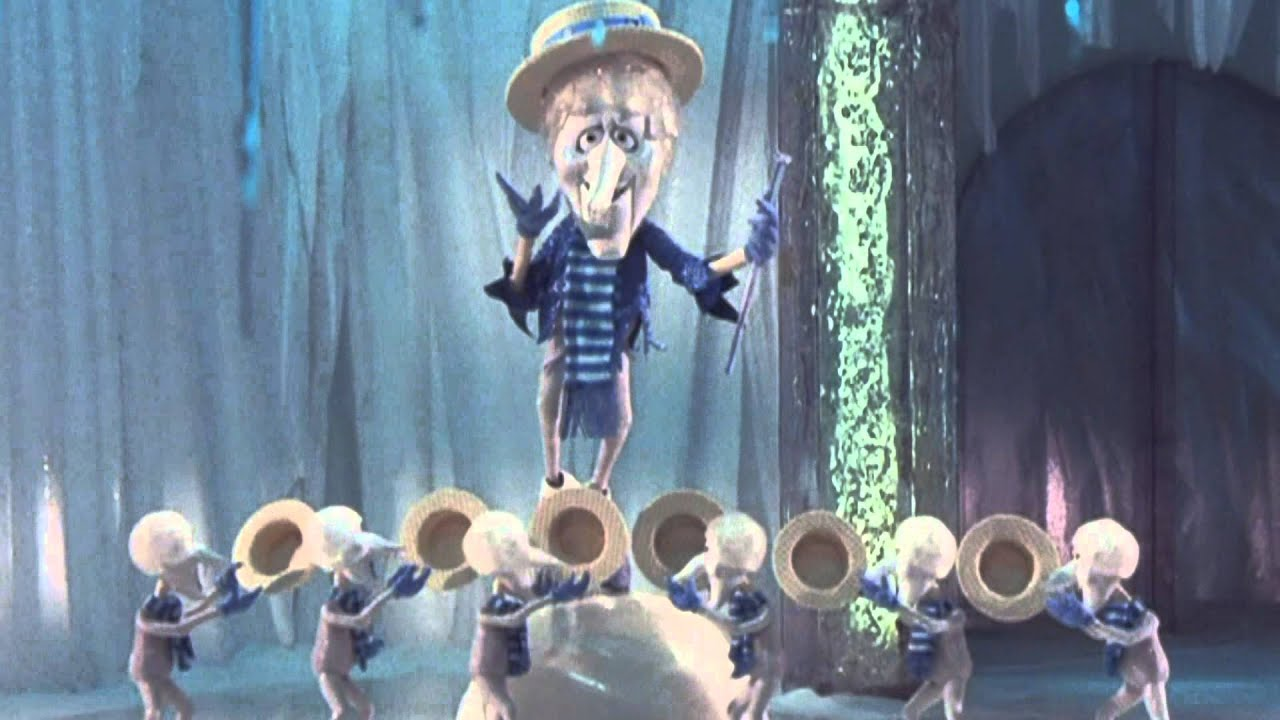
\includegraphics[width=0.9\textwidth]{snow-miser.jpg}
  \end{frame}

  \begin{frame}
    \frametitle{Not So Fast!}

    \begin{itemize}
      \item We're not quite in AI winter terrritory yet! There were some
        important achievements from the mid-60s to the 70s.
      \pause
      \item Early face recognition (Woody Bledsoe, Takeo Kanade et al.).
      \pause
      \item Three-dimensional object recognition (Lawrence G. Roberts, Seymour
        Papert et al.).
      \pause
      \item Image filtering methods still used today (e.g. the Sobel-Feldman
        operator).
      \pause
      \item A slow, crappy robot called Shakey.
      \pause
      \item SHRDLU.
      \pause
      \item DENDRAL.
    \end{itemize}
  \end{frame}

  \begin{frame}
    \frametitle{AI Winter(s, Plural)}

    \begin{itemize}
      \item From the 60s to the 80s several hype cycles resulted in AI winter
        events. These were caused by:
      \pause
      \item The ALPAC report of 1966.
      \pause
      \item The publication of \textit{Perceptrons} in 1969.
      \pause
      \item The Lighthill report of 1973.
      \pause
      \item US researchers somehow managing to exhaust (D)ARPA's patience.
      \pause
      \item The failed Fifth Generation Computer Systems initiative from
        Japan.
      \pause
      \item Excess optimism towards expert systems deflating.
      \pause
      \item Further cutbacks to DARPA initiatives.
      \pause
      \item The collapse of the Lisp machine market.
    \end{itemize}
  \end{frame}

  \subsection{Early Modern Methods}

  \begin{frame}
    \frametitle{A Quick Introduction}

    \begin{itemize}
      \item About the term ``early modern'': I stole it from world history.
        It's not official.
      \pause
      \item I'm going to be pretty brief in this subsection and the next
        because this is stuff you probably already mostly know about. I don't
        want to seem patronizing.
    \end{itemize}
  \end{frame}

  \begin{frame}
    \frametitle{80s Comeback}

    \begin{itemize}
      \item AI had quite a boom in the 80s!
      \pause
      \item Although a lot of the renewed interest in AI ultimately led to the
        failures and disappointments described previously, but some of the
        initiatives had staying power.
      \pause
      \item The most iconic achievement of this decade in the domain of AI was
        the popularization of connectionism. (Be sure to bring up Yann LeCun's
        research for the USPS.)
      \pause
      \item Semantic networks and the curious case of Doug Lenat.
      \pause
      \item Decision trees!
    \end{itemize}
  \end{frame}

  \begin{frame}
    \frametitle{AI from 1993 to 2011: A Highlights Reel}

    \begin{itemize}
      \item Most of the successes from this period seem to have more to do
        with application of existing theoretical knowledge rather than
        fundamental breakthroughs. (Not that those aren't needed too! I'm bad
        at theory!)
      \pause
      \item Euphemisms (``computational intelligence'' etc.) were used to
        ensure that practical work focused on short-term goals could receivve
        funding. (Mention the Nick Bostrom quote.)
      \pause
      \item Hardware improvements finally make solid ideas feasible in
        practice, Deep Blue being a good example.
      \pause
      \item DARPA Grand Challenge victory (2005, 131 miles), DARPA Urban
        Challenge (2007, 55 miles).
      \pause
      \item In 2011, Watson stomps Brad Rutter and Ken Jennings in
        \textit{Jeopardy!}.
      \pause
      \item ``Where is HAL 9000?'' Various answers from Minsky, McCarthy,
        Kurzweil and Hawkins.
      \pause
      \item Bonus item: the Apriori association rule learning algorithm,
        though not the first of its kind, was described in 1993 and the paper
        by Agrawal et al. has over 21,000 citations on Google Scholar, making
        it one of the most cited papers in the field!
    \end{itemize}
  \end{frame}

  % Prelude
  % Supervised, unsupervised
  % Emphasize relative simplicity of many algorithms

  \subsection{Deep Learning}

  \section{Assessing Realisticness of Applications}

  \subsection{Overview}

  \begin{frame}
    \frametitle{Overview}

    \begin{itemize}
      \item Broadly speaking, the current tendency in our society is to
        overestimate what is possible with the state of the art in AI rather
        than to underestimate it. Accordingly, indicating where AI is
        currently particularly weak can bring about a more realistic
        appraisal.
      \pause
      \item At the same time, we don't want to go too far. Think about a
        prospect like near-native translation between any two languages in
        text or audio. We don't have it but I could see that happening in the
        near future perhaps. Generally, you should at least already have some
        idea of what is \emph{currently} feasible so I won't spend any more
        time talking about that
      \pause
      \item I like to use lots of analogies and stories instead of getting
        bogged down in technical details when I explain these sorts of things
        and I think I've included a few of my best here. You be the judge!
    \end{itemize}
  \end{frame}

  \subsection{The Current Hurdles to Perfection}

  % Domain specificity vs. domain generality (might want to make mention of
  % ACT-R or other attempts at more domain generality?)
  % Olympics analogy for no free lunch theorem
  % Steam locomotive analogy
  % Was the lethal police robot really a robot?
  % Objection from Singularitarianism: Anecdote about number factoring
  % Rodney Brooks' argument about evolution
  % No data, no success

  \section{The Geography of AI Development}
  \section{Impacts on Employment}
  \section{Future of Human-AI Interaction}
  \section{Impact on Philosophy and Religion}
  % Mention kami before 40K
  \section{Impact on Ethics}
  \section{AI and Statistical Literacy}
  \section{Recommended Media}
  % Quest for Artificial Intelligence
  
  \begin{comment}
Subject: Communicating AI Effectively

Possible topics (will likely have to pare them down due to time limitations):

* Taxonomy of AI and its uses:

** Different methods, both at the level of categories (e.g. supervised
learning), and concrete methods (e.g. k-NN). These are most popular these days
but can also be contrasted with traditional methods such as tree search that
dominate texts like Artificial Intelligence: A Modern Approach.

** Applications of these methods (NLP, image classification, computer
opponents, recommender systems, etc.).

* What's realistic and what's not realistic. I'd probably only call anything
involving something like hypercomputation impossible but a lot of things are
just really most likely not going to happen. This would include anything like
Skynet. (This has long been difficult even for luminaries in the field. For
example when Logic Theorist was created and came up with better proofs for
theorems in Principia Mathematica (the Russell and Whitehead one, not the
Newton one) than the human authors, this led to enthusiastic thinking that
human-level or better artificial intelligence would appear in a few decades.
This did not happen.) Of course for all but one of you I am now beating a dead
horse but the most likely path to the superhuman is an enhanced human rather
than something built from scratch. This may or may not include integration of
artificially intelligent components with the human body.

* Assessment of strengths in development and use of AI technology by country /
region. Primarily this means comparing the USA and PRC. Japan (as well as the
broader Jakota triangle of Japan, ROK and Taiwan), Western Europe, India and
Israel also merit some attention.

* How structural unemployment is likely to play out. ("You will almost
certainly be far safer as a roofer than as a legal researcher...")

* Impact of human-AI interaction in the future. (Japan being a very good
example.)

* Impact of AI and other GRIN (genetic, robotic, information technology,
nanotechnology) technologies on religions and other belief systems. "Dataism"
as put forward by Yuval Noah Harari leading example. Possible compatibility of
traditional religious thinking with mechanistic ideas of the mind typical in
cognitive science assessed as well: Descartes and Hobbes had mechanistic ideas
of the mind and at least one of them (Descartes) was almost definitely a
sincere believer. (Hobbes may have been a closeted atheist.) Japanese notion
of kami where entities not usually considered to have a spirit by other people
also highly relevant—priority of making robots human-like in Japan not likely
coincidental. Fictional examples like the Machine Cult from the card game Star
Realms and Meklar species from the Master of Orion games also worth mentioning
because they reflect on what we think might happen someday.

* Recommended reading / people: both of Yuval Noah Harari's future-oriented
books and The Master Algorithm by Pedro Domingos stand out in my mind
particularly. I also have a high opinion of The Deep Learning Revolution by
Terrence J. Sejnowski. Kinda ambivalent about Weapons of Math Destruction by
Cathy O'Neill because I think the ideological slant ends up in points that
aren't very good in some places but it's still worth a read. Heard good things
about Kai-Fu Lee's book but haven't read it yet. I've read and heard a lot
from Rodney Brooks and generally he's very on point as is another roboticist,
Rolf Pfeifer. Also look into the ideas of J.C.R. Licklider, who was ahead of
the curve by decades—Man-Computer Symbiosis was published in 1960.

* Statistical literacy—most of what we now call "AI" is heavily dependent on
statistics. More technical but includes things like knowing that a p-value is
a conditional probability, statistical vs. practical significance, why one
shouldn't do a whole bunch of significance tests without correcting for
multiple comparisons, frequentism vs. Bayesianism etc.

* Machine ethics: who will get run over by an autonomous car if there is no
other option? Goes into how Isaac Asimov's famous Laws of Robotics don't
really work. (He knew this and often exploited it in his writing.) Military is
of course another issue. There's an interesting book about this, Governing
Lethal Behavior in Autonomous Robots by Ronald C. Arkin. The methods proposed
are kind of high-level and hand-wavey but he does a lot to integrate
traditional Western ethics of war with current prospects of warfighting
machines. Other legal issues. What the technology should be used for.
  \end{comment}
\end{document}
